\documentclass[10pt]{beamer}
\setbeamertemplate{navigation symbols}{\insertlogo}

%\documentclass[handout,dvips,11pt,grey]{beamer}

%\usetheme{Goettingen}
%\usetheme{Warsaw}
\usetheme{Hannover}

%\usepackage{tikz,pgf}
\usepackage{multicol}
\usepackage{amsmath,amsthm,amssymb}
%\usepackage{epstopdf}
%\usepackage{xspace}
\usepackage{wrapfig}

\usepackage{verbatim}
%\usepackage{circuitikz}
%\usepackage{graphicx}
\usepackage{comment}
%\usepackage{array}
\usepackage{coffee4}

\title{Identifying Subject Matter Experts}
\subtitle{Extending Author Topic Modeling}
\author{Philip Robinson}
\date{\today}
\institute{Presented to OCIO \\ NASA - Jet Propulsion Lab}

\DeclareMathOperator*{\argsort}{argsort}

  \logo{
\includegraphics[height=.7cm]{./logo.png}}


\begin{document}

\begin{frame}
  \titlepage


\end{frame}

\section{Introduction}
\begin{frame}{Introduction - Philip Robinson}
  Computer Science MSc at Oregon Health and Science University.

  \vspace{1em}

  {\em Thanks to my mentor Ian Colwell, from the OCIO (1762)}

  \begin{multicols}{2}
    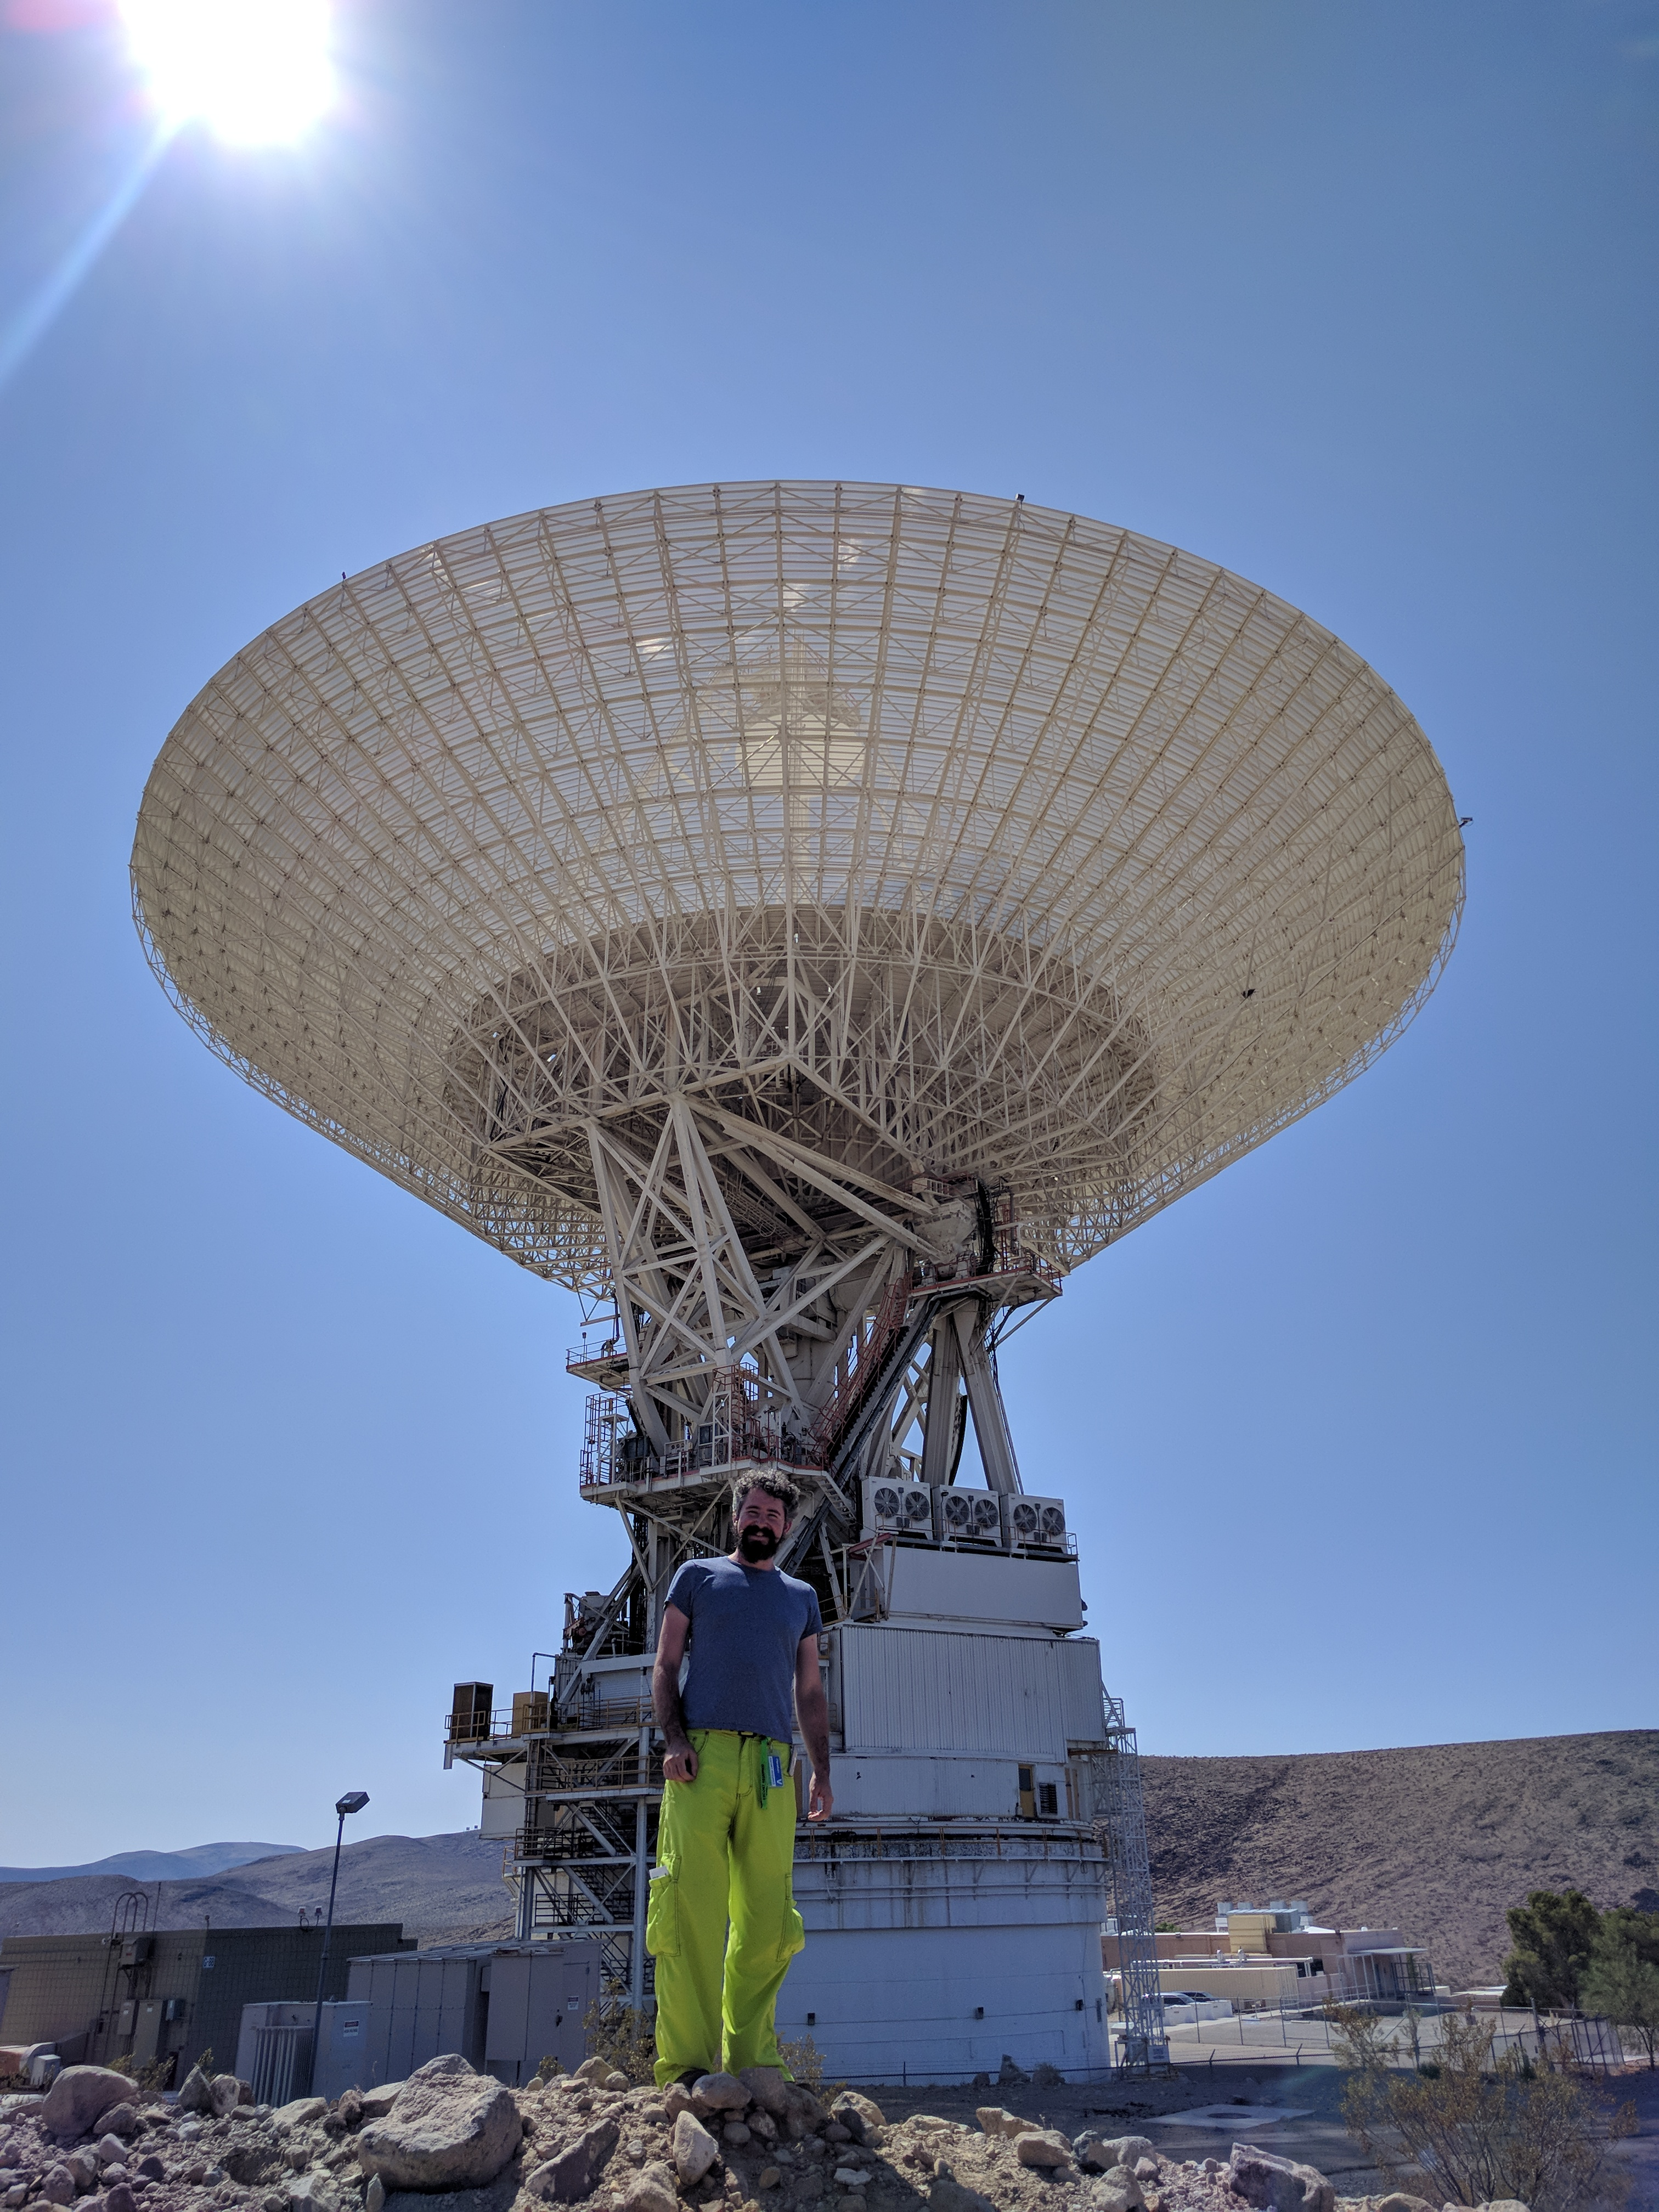
\includegraphics[width=\columnwidth]{./philip.jpg}

    \begin{itemize}
    \item probabilistic programming
    \item language processing
    \item image processing
    \item audio processing
    \item stem education
    \item environmental sciences
    \end{itemize}

  \end{multicols}

\end{frame}

\begin{frame}{Presentation Overview}
  \tableofcontents

\end{frame}



\section{Problem Description}

\begin{frame}{Problem Description}
  Our customers, Office of Safety and Mission Success (5x), are interested in
  identifying experts for resolving anomaly reports in the Problem Reporting System (PRS)

  \vspace{2em}

  % meditate on including prior work
  OCIO (17x) has been previously asked for subject matter expert
  identification systems and document similarity tools, so show
  particular interest is solutions that provide similarity metrics
  and can generalize to other teams and corpora.


  \begin{itemize}
  \item A-Team heirarchical frequent item set expert exploration tool
  \item TechConnect self reported skills host
  \item Gateway Profiles
  \end{itemize}
\end{frame}

\begin{frame}{Motivating Story}
  \begin{itemize}
  \item Domain experts are lost between projects
  \item Domain experts are often coupled to a single project
  \item Very few candidates resolve the majority of tickets
  \end{itemize}

    \begin{itemize}
  \item Expert discoverability
  \item Load balancing employees
  \item Identification of knowledge gaps
  \end{itemize}


\end{frame}

\begin{frame}{Objective}
  \begin{itemize}
  \item Assign \& Resolve anomalies quicker
  \item Support queries for expert discovery
  \item Find employees with similar domain expertise
%  \item Identify knowledge gaps against a corpus
  \end{itemize}
\end{frame}



\begin{frame}{Data Provided for Internship}
  \begin{itemize}
  \item Problem Reporting System (Anomalies)
    \begin{itemize}
    \item Problem Failure Report (PFR)
    \item Developmental Problem Failure Report (DPFR)
    \item Incident Surprise Anomaly (ISA)
    \end{itemize}
  \end{itemize}

  \hrulefill
  \begin{itemize}
  \item Free Text
    \begin{itemize}
    \item Title
    \item Description
    \end{itemize}
  \item Experts
    \begin{itemize}
    \item Responsible Editor
    \item Assignee
    \end{itemize}
  \end{itemize}
\end{frame}


%\begin{frame}{Terms}
%\end{frame}

\section{Proposed Approach}

\begin{frame}{Approach - Topic Modeling}

% Fitting authorship as a generative model allows us to mathematically abstract and describe a provided corpus, allowing us to ask deeper questions about incoming documents. We elect using the Author-Topic-Model (ATM) to ask the `most likely author' of a document, as a proxy for expertise.

  \begin{multicols}{2}

  \begin{itemize}
  \item Interpret doc as BOW\footnote{Bag of Words}
  \item Model/Fit topics as mixture of words
  \item Author \& document are projected into topic-space
  \item Measure distance from author to document
  \end{itemize}

  \begin{figure}
  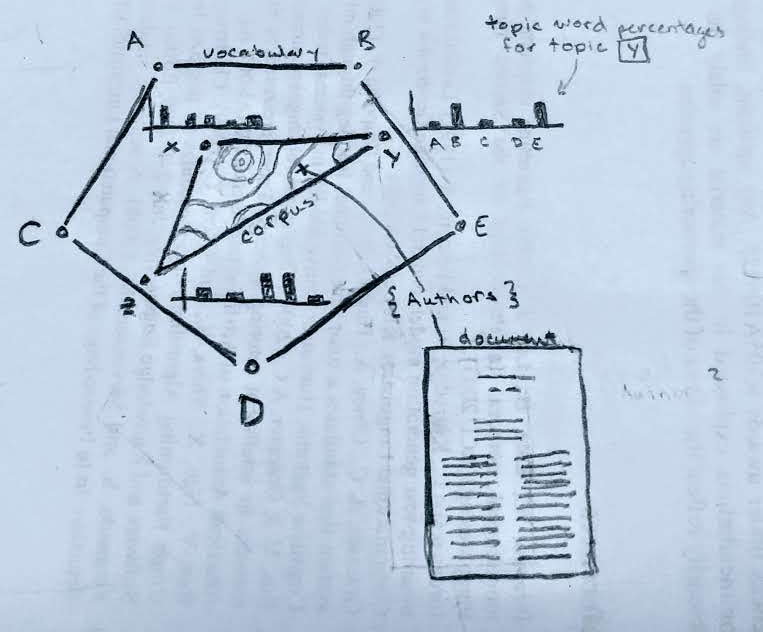
\includegraphics[width=\columnwidth]{./lda-draw.jpg}
  \caption{Latent Dirichlet Allocation}
  \end{figure}

  \end{multicols}

  \begin{align*}
    T(x) &= \texttt{Project $x$ into topic-space} \\
    R_d &= \argsort_{a\in A} \left\{Distance(T(a),T(d))\right\}
  \end{align*}

\end{frame}


\begin{comment}
\section{Details}


\begin{frame}{Text Pre-Processing}

  ATM is a derivative of Latent Dirichlet Allocation (LDA), which is a generative \texttt{bag-of-words} model for producing topics described as a mixture of words.

  \begin{itemize}
  \item Join all Free Text fields
  \item Lowercase text
  \item Remove non-informative text patterns
  \item Stem \hfill\texttt{(applies, applying, apply) -> (appli)}
  \item Un-Stem \hfill\texttt{(appli) -> (apply)}
  \item Identify and remove ``Stop Words''
    \begin{itemize}
    \item most frequent .06\% (empirical choice)
    \item \texttt{nltk} english stop-words
    \end{itemize}
  \item Remove rare words
  \end{itemize}

\end{frame}


\begin{frame}{Document Selection}
  LDA has some performance restrictions, like not handling short documents well.
  \begin{itemize}
  \item Remove short documents
  \item Remove documents with high stop-word ratio
  \end{itemize}
\end{frame}


\end{comment}

\begin{frame}{Latent Dirichlet Allocation (LDA)}
  LDA is a generative model that describes each document as a mixture of topics, and each topic as a mixture of words.
  %These topics are not always interpretable, but have interesting mathematical properties.
  %For our purposes LDA acts as a dimensionality reduction technique. We project documents from a ``Vocabulary Space'' to a ``Topic Space'', from dimension  $\sim50000$ to $\sim60$.

  \vspace{1em}

\begin{multicols}{2}
    \begin{itemize}
    \item Tune hyper-parameters %\texttt{(iterations, count-topics, $\alpha$)}
      \begin{itemize}
      \item[ISA] 351 iterations, 40 topics
      \item[PFR] 251 iterations, 25 topics
      \item[DPFR] 351 iterations, 25 topics
      \end{itemize}
      \columnbreak
    \item Measures
    \begin{itemize}
    \item Perplexity (statistic)
    \item Coherence (statistic)
    \item Visualizations (exploratory)
    \end{itemize}
    \end{itemize}


\end{multicols}

    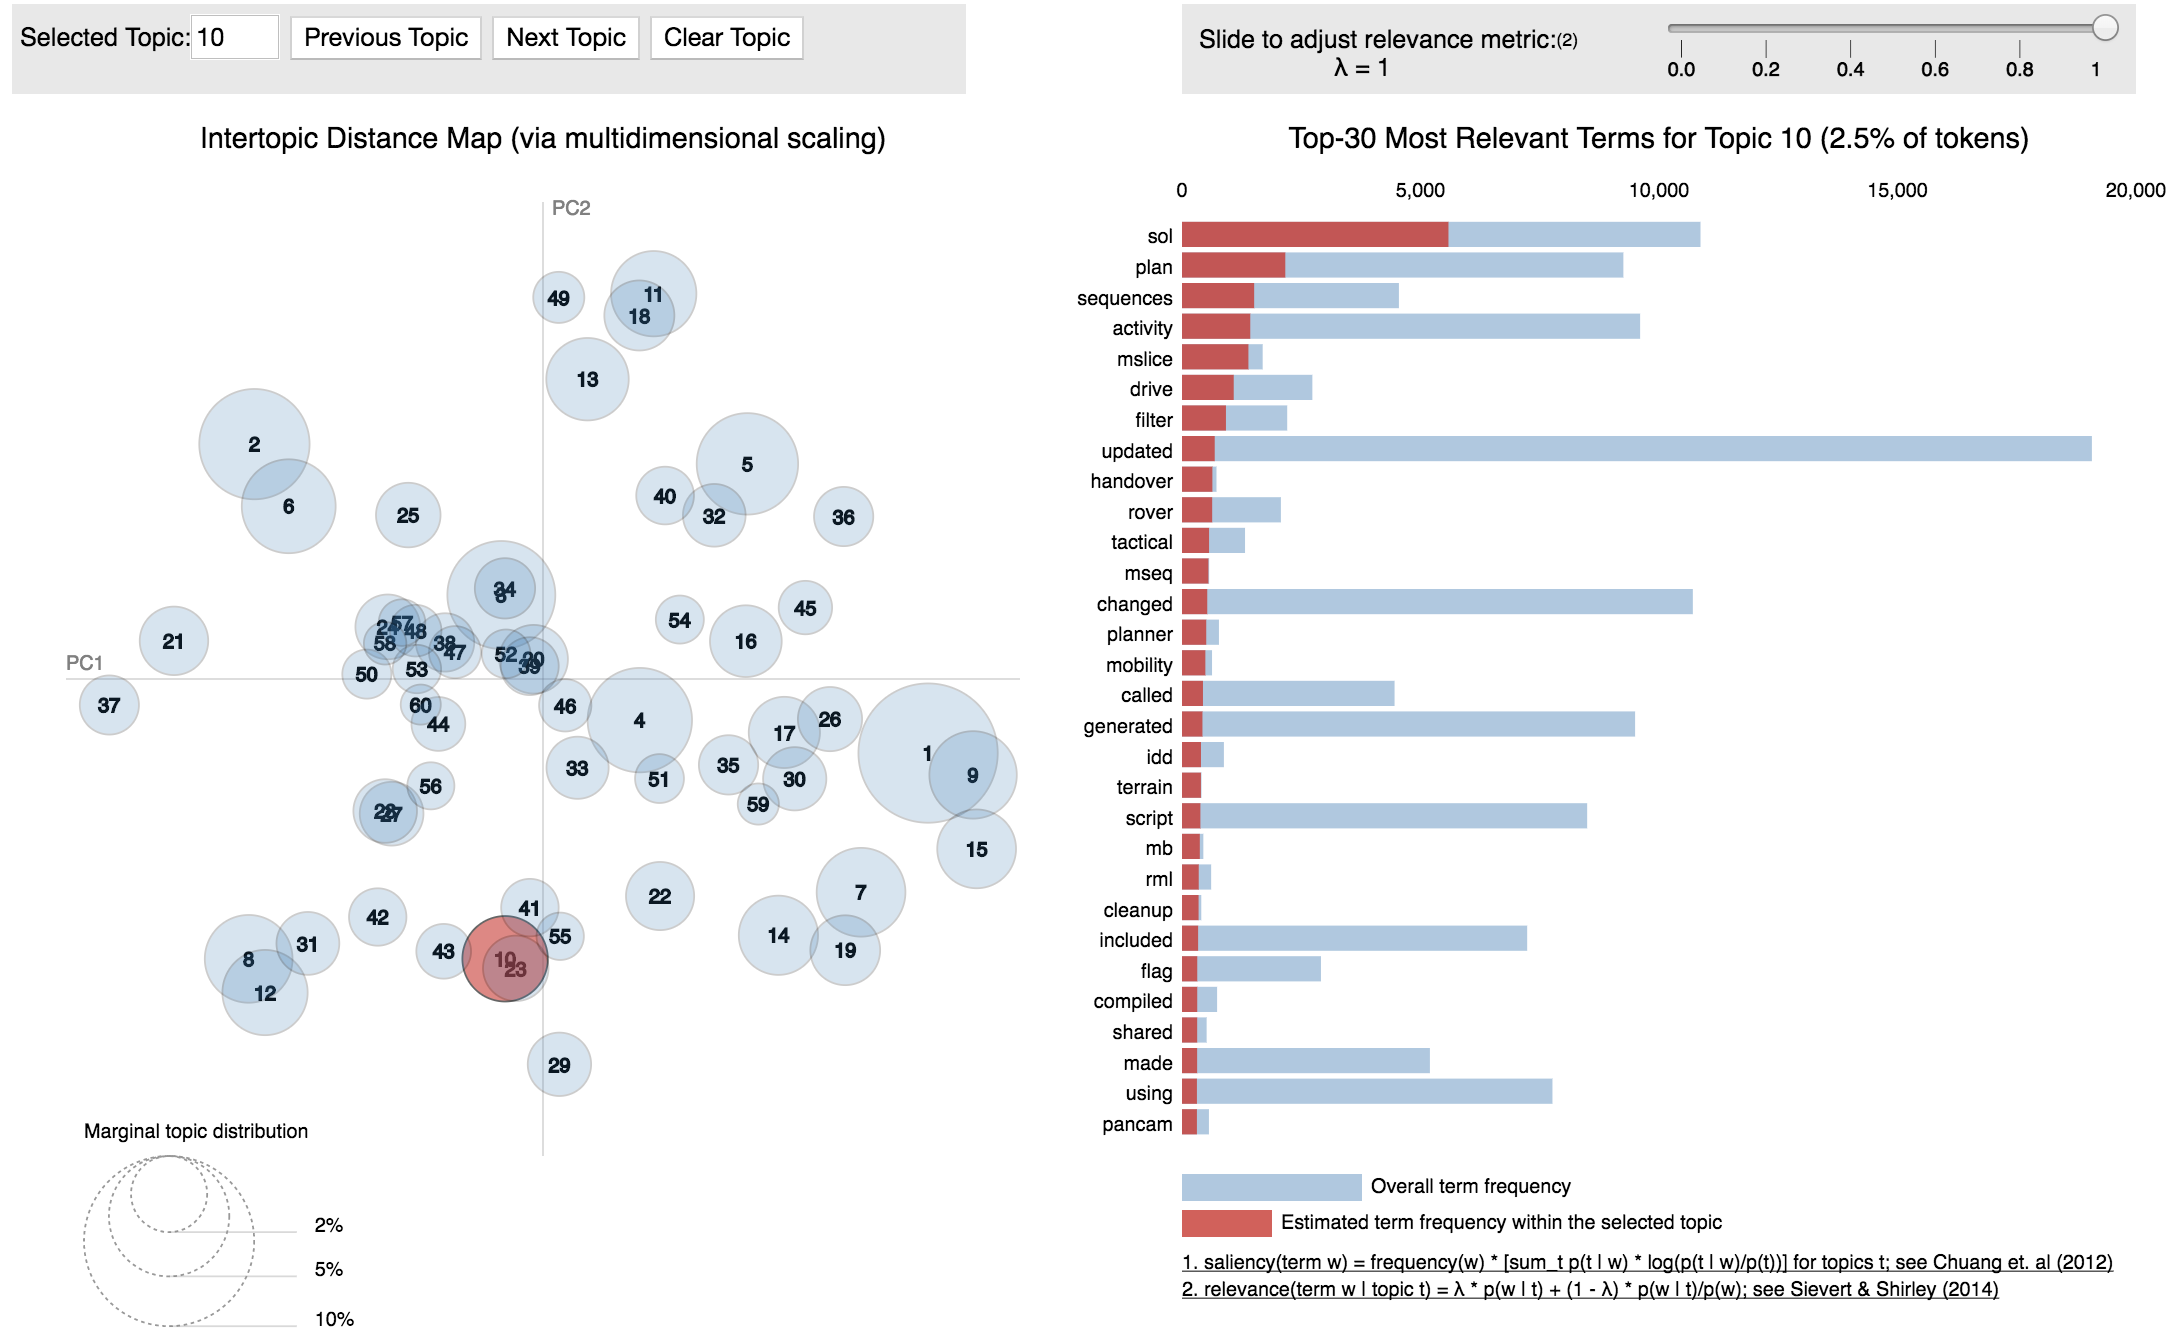
\includegraphics[width=0.6\textwidth]{LDAvis.png}

\end{frame}

\begin{frame}{Author Topic Model}

  ATM extends LDA to describe authors as a mixture of topics. This allows us to ask questions relating to both documents and authors. Both documents and authors are now mapped to the ``Topic Space'' described in LDA.

  \begin{itemize}
  \item Down sample to documents with a Responsible Editor / Assignee
  \item Split into Train and Validation
  \item Train model
  \end{itemize}

\end{frame}

\begin{frame}{Ranking}

  Given Authors/Experts in a ``Topic Space'' and a mapping from document to ``Topic Space'', we can rank likely authors for a document. Ideally this is done with the probability of an author given a document, but presently we use distribution similarity metrics to rank authors.

  \begin{itemize}
  \item Elect a similarity metric \texttt{(Hellinger Distance)}
  \item Rank likely authors on Train and Test document sets
  \item Inspect/Present results
  \end{itemize}

  \begin{multicols}{2}
    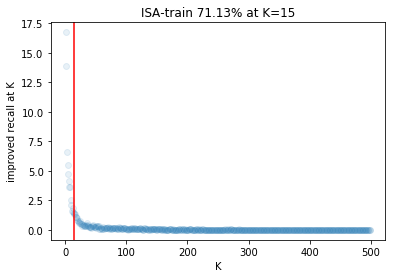
\includegraphics[width=\columnwidth]{./recall-train-isa.png}

    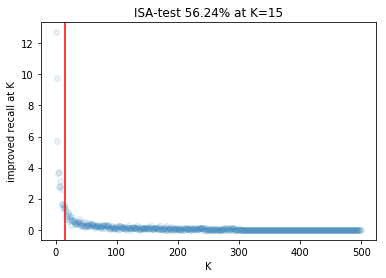
\includegraphics[width=\columnwidth]{./recall-test-isa.png}
  \end{multicols}

  K is cutoff for suggested candidates
\end{frame}

\section{Investivation}

\begin{frame}{Does publication count effect recall?}

  {\bf Nope; and thats good}
%  These plots show the ranking of True authors, against a provided document. The \texttt{x-axis} tells us how many publications were attributed to a author, the \texttt{y-axis} tells us what rank they received when evaluated against the specific document. The darkness of a hexblock indicates the population density of an \texttt{(X,Y)} location, like a heatmap. A dark line along the \texttt{Y=0} is a strong indicator that this process is behaving as expected.

  % NEED TO EXPLAIN THIS PLOT

  %It is reasonable to be suspicious that candidates that work on a large number of tickets would be much easier to identify, than those who work on few.
  This plot shows consistent identification distribution as a function of publication count from the train set.

  \begin{multicols}{2}
    Train
    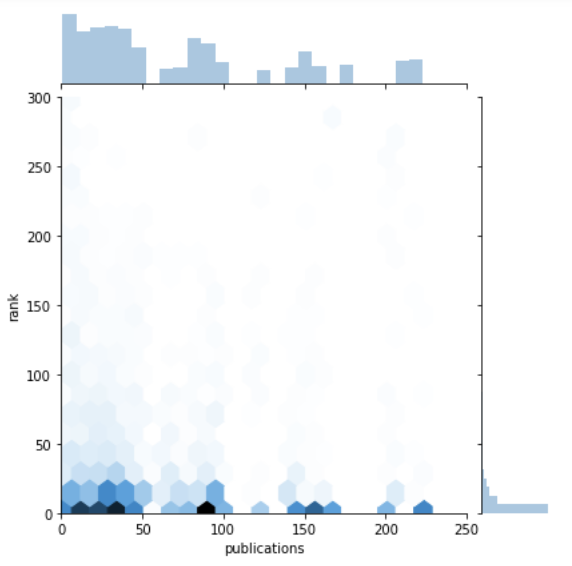
\includegraphics[width=\columnwidth]{./Train.png}

    Test
  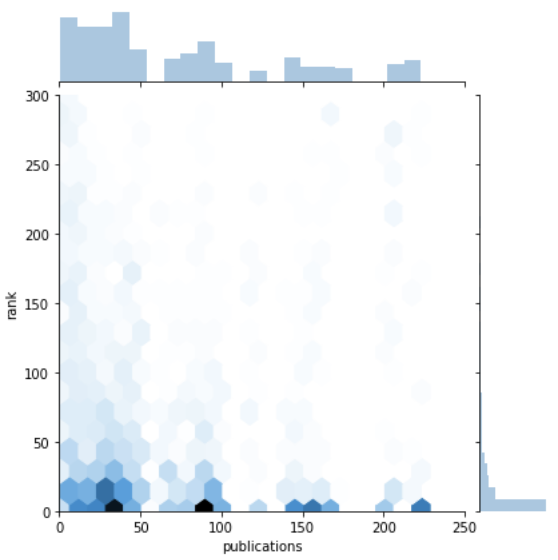
\includegraphics[width=\columnwidth]{./Test.png}
  \end{multicols}
\end{frame}


\begin{frame}{How does word count effect recall?}

  {\bf Best results at 30 words}

  We are interested in understanding how much text is required to inform
  our model prediction. For these plots, we randomly subset texts for
  known ticket-expert pairs and observe the expert's new ranking.

  \begin{multicols}{2}
    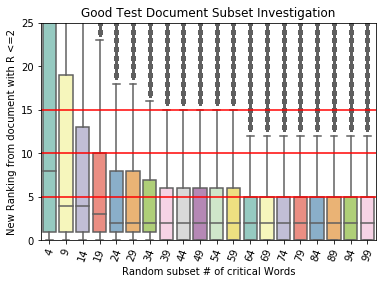
\includegraphics[width=\columnwidth]{low-ranked-downsample.png}
    Expert found in top 2\\
    24 critical words


    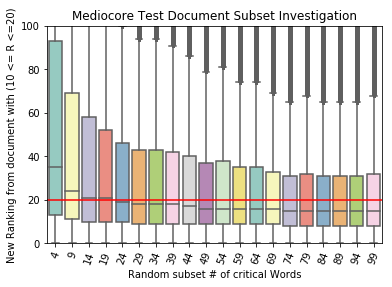
\includegraphics[width=\columnwidth]{mid-ranked-downsample.png}
    expert found in 10-20 range\\
    29 critical words
  \end{multicols}
\end{frame}

\section{Results}

\begin{frame}{Results}

  It is possible to get interesting results at a document length of 4 words,
  however it is hard to know why these results are interesting.
  This is an example of directly searching for experts.

  \begin{multicols}{2}
    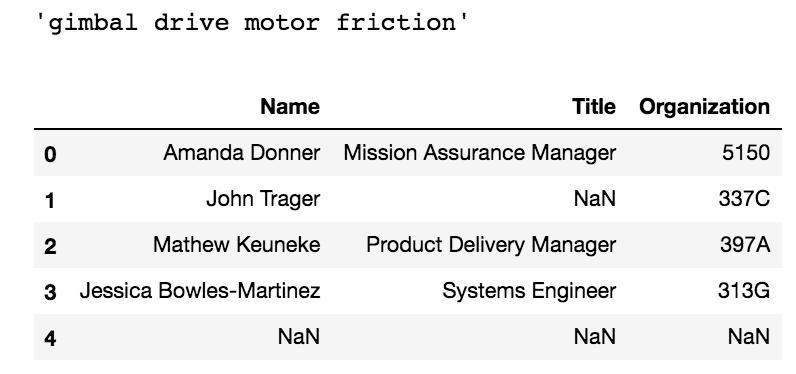
\includegraphics[width=\columnwidth]{query1.png}

    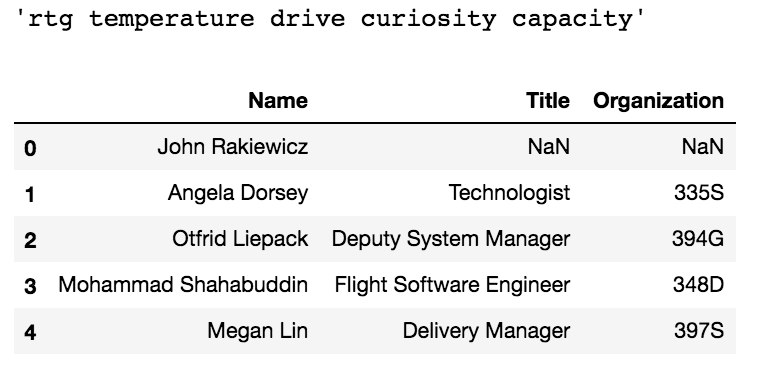
\includegraphics[width=\columnwidth]{query2.png}
  \end{multicols}

  Documents queries generate better results. These examples are
  currently unable to demo.

\end{frame}

\begin{frame}{Next Steps}
  \begin{itemize}
  \item Extend tool to provide visualizations supporting for ranking
  \item Build UI for testing and authoring documents
  \item Contact high ranked persons to verify expertise
  \item Filter based on job title
  \item Open Sourcing
  \end{itemize}

\end{frame}

\section{Conclusion}

\begin{frame}{Conclusion}
  \begin{itemize}
  \item This looks like it works
  \item Not computationally or socially prohibitive
  %\item This can be implemented as an On-Line model thanks to Variational Bayes Sampling
  \item Motivating story to lift limitations on data access
  \item Further investigation is needed to insure best expert fields
  \item User interface is required for integration into workflows
  \end{itemize}
\end{frame}


\begin{frame}{Internship Notes}
  I had never implemented a recommender system, nor used topic modeling in
  a project prior to this task. I will be leaving JPL with a holistic understanding
  of topic modeling, and a much better understanding of recommender systems.

\vspace{1em}

  This work has encouraged me to look at continued employment in applications of
  machine learning for information retrieval more realistically. I'm also interested
  in keeping in touch over future employment opportunities with JPL.

  \vspace{1em}

  Having multiple interns work with the same data helps. We were able to work through
  data difficulties together, and share results.
\end{frame}


\begin{frame}{Thanks}
  I received a lot of input in for this project from my team.
  Their insight, especially, bridged the gap from academic to practical evaluation of models,
  and I sincerely appreciate their contributions.

  \begin{itemize}
  \item Ian Colwell
  \item Valentinos Constantinou
  \item Jerry Chen
  \item Leslie Callum
  \item Bruce Waggoner
  \item Harald Schone
  \item Chris Mattmann
  \item[] et. al.
  \end{itemize}

\end{frame}

\end{document}
